% Options for packages loaded elsewhere
\PassOptionsToPackage{unicode}{hyperref}
\PassOptionsToPackage{hyphens}{url}
\PassOptionsToPackage{dvipsnames,svgnames,x11names}{xcolor}
%
\documentclass[
  letterpaper,
  DIV=11,
  numbers=noendperiod]{scrartcl}

\usepackage{amsmath,amssymb}
\usepackage{iftex}
\ifPDFTeX
  \usepackage[T1]{fontenc}
  \usepackage[utf8]{inputenc}
  \usepackage{textcomp} % provide euro and other symbols
\else % if luatex or xetex
  \usepackage{unicode-math}
  \defaultfontfeatures{Scale=MatchLowercase}
  \defaultfontfeatures[\rmfamily]{Ligatures=TeX,Scale=1}
\fi
\usepackage{lmodern}
\ifPDFTeX\else  
    % xetex/luatex font selection
\fi
% Use upquote if available, for straight quotes in verbatim environments
\IfFileExists{upquote.sty}{\usepackage{upquote}}{}
\IfFileExists{microtype.sty}{% use microtype if available
  \usepackage[]{microtype}
  \UseMicrotypeSet[protrusion]{basicmath} % disable protrusion for tt fonts
}{}
\makeatletter
\@ifundefined{KOMAClassName}{% if non-KOMA class
  \IfFileExists{parskip.sty}{%
    \usepackage{parskip}
  }{% else
    \setlength{\parindent}{0pt}
    \setlength{\parskip}{6pt plus 2pt minus 1pt}}
}{% if KOMA class
  \KOMAoptions{parskip=half}}
\makeatother
\usepackage{xcolor}
\setlength{\emergencystretch}{3em} % prevent overfull lines
\setcounter{secnumdepth}{5}
% Make \paragraph and \subparagraph free-standing
\ifx\paragraph\undefined\else
  \let\oldparagraph\paragraph
  \renewcommand{\paragraph}[1]{\oldparagraph{#1}\mbox{}}
\fi
\ifx\subparagraph\undefined\else
  \let\oldsubparagraph\subparagraph
  \renewcommand{\subparagraph}[1]{\oldsubparagraph{#1}\mbox{}}
\fi

\usepackage{color}
\usepackage{fancyvrb}
\newcommand{\VerbBar}{|}
\newcommand{\VERB}{\Verb[commandchars=\\\{\}]}
\DefineVerbatimEnvironment{Highlighting}{Verbatim}{commandchars=\\\{\}}
% Add ',fontsize=\small' for more characters per line
\usepackage{framed}
\definecolor{shadecolor}{RGB}{241,243,245}
\newenvironment{Shaded}{\begin{snugshade}}{\end{snugshade}}
\newcommand{\AlertTok}[1]{\textcolor[rgb]{0.68,0.00,0.00}{#1}}
\newcommand{\AnnotationTok}[1]{\textcolor[rgb]{0.37,0.37,0.37}{#1}}
\newcommand{\AttributeTok}[1]{\textcolor[rgb]{0.40,0.45,0.13}{#1}}
\newcommand{\BaseNTok}[1]{\textcolor[rgb]{0.68,0.00,0.00}{#1}}
\newcommand{\BuiltInTok}[1]{\textcolor[rgb]{0.00,0.23,0.31}{#1}}
\newcommand{\CharTok}[1]{\textcolor[rgb]{0.13,0.47,0.30}{#1}}
\newcommand{\CommentTok}[1]{\textcolor[rgb]{0.37,0.37,0.37}{#1}}
\newcommand{\CommentVarTok}[1]{\textcolor[rgb]{0.37,0.37,0.37}{\textit{#1}}}
\newcommand{\ConstantTok}[1]{\textcolor[rgb]{0.56,0.35,0.01}{#1}}
\newcommand{\ControlFlowTok}[1]{\textcolor[rgb]{0.00,0.23,0.31}{#1}}
\newcommand{\DataTypeTok}[1]{\textcolor[rgb]{0.68,0.00,0.00}{#1}}
\newcommand{\DecValTok}[1]{\textcolor[rgb]{0.68,0.00,0.00}{#1}}
\newcommand{\DocumentationTok}[1]{\textcolor[rgb]{0.37,0.37,0.37}{\textit{#1}}}
\newcommand{\ErrorTok}[1]{\textcolor[rgb]{0.68,0.00,0.00}{#1}}
\newcommand{\ExtensionTok}[1]{\textcolor[rgb]{0.00,0.23,0.31}{#1}}
\newcommand{\FloatTok}[1]{\textcolor[rgb]{0.68,0.00,0.00}{#1}}
\newcommand{\FunctionTok}[1]{\textcolor[rgb]{0.28,0.35,0.67}{#1}}
\newcommand{\ImportTok}[1]{\textcolor[rgb]{0.00,0.46,0.62}{#1}}
\newcommand{\InformationTok}[1]{\textcolor[rgb]{0.37,0.37,0.37}{#1}}
\newcommand{\KeywordTok}[1]{\textcolor[rgb]{0.00,0.23,0.31}{#1}}
\newcommand{\NormalTok}[1]{\textcolor[rgb]{0.00,0.23,0.31}{#1}}
\newcommand{\OperatorTok}[1]{\textcolor[rgb]{0.37,0.37,0.37}{#1}}
\newcommand{\OtherTok}[1]{\textcolor[rgb]{0.00,0.23,0.31}{#1}}
\newcommand{\PreprocessorTok}[1]{\textcolor[rgb]{0.68,0.00,0.00}{#1}}
\newcommand{\RegionMarkerTok}[1]{\textcolor[rgb]{0.00,0.23,0.31}{#1}}
\newcommand{\SpecialCharTok}[1]{\textcolor[rgb]{0.37,0.37,0.37}{#1}}
\newcommand{\SpecialStringTok}[1]{\textcolor[rgb]{0.13,0.47,0.30}{#1}}
\newcommand{\StringTok}[1]{\textcolor[rgb]{0.13,0.47,0.30}{#1}}
\newcommand{\VariableTok}[1]{\textcolor[rgb]{0.07,0.07,0.07}{#1}}
\newcommand{\VerbatimStringTok}[1]{\textcolor[rgb]{0.13,0.47,0.30}{#1}}
\newcommand{\WarningTok}[1]{\textcolor[rgb]{0.37,0.37,0.37}{\textit{#1}}}

\providecommand{\tightlist}{%
  \setlength{\itemsep}{0pt}\setlength{\parskip}{0pt}}\usepackage{longtable,booktabs,array}
\usepackage{calc} % for calculating minipage widths
% Correct order of tables after \paragraph or \subparagraph
\usepackage{etoolbox}
\makeatletter
\patchcmd\longtable{\par}{\if@noskipsec\mbox{}\fi\par}{}{}
\makeatother
% Allow footnotes in longtable head/foot
\IfFileExists{footnotehyper.sty}{\usepackage{footnotehyper}}{\usepackage{footnote}}
\makesavenoteenv{longtable}
\usepackage{graphicx}
\makeatletter
\def\maxwidth{\ifdim\Gin@nat@width>\linewidth\linewidth\else\Gin@nat@width\fi}
\def\maxheight{\ifdim\Gin@nat@height>\textheight\textheight\else\Gin@nat@height\fi}
\makeatother
% Scale images if necessary, so that they will not overflow the page
% margins by default, and it is still possible to overwrite the defaults
% using explicit options in \includegraphics[width, height, ...]{}
\setkeys{Gin}{width=\maxwidth,height=\maxheight,keepaspectratio}
% Set default figure placement to htbp
\makeatletter
\def\fps@figure{htbp}
\makeatother

% load packages
\usepackage{geometry}
\usepackage{xcolor}
\usepackage{eso-pic}
\usepackage{fancyhdr}
\usepackage{sectsty}
\usepackage{fontspec}
\usepackage{titlesec}

%% Set page size with a wider right margin
\geometry{a4paper, total={170mm,257mm}, left=20mm, top=20mm, bottom=20mm, right=50mm}

%% Let's define some colours
\definecolor{light}{HTML}{E6E6FA}
\definecolor{highlight}{HTML}{800080}
\definecolor{dark}{HTML}{330033}

%% Let's add the border on the right hand side 
\AddToShipoutPicture{% 
    \AtPageLowerLeft{% 
        \put(\LenToUnit{\dimexpr\paperwidth-3cm},0){% 
            \color{light}\rule{3cm}{\LenToUnit\paperheight}%
          }%
     }%
     % logo
    \AtPageLowerLeft{% start the bar at the bottom right of the page
        \put(\LenToUnit{\dimexpr\paperwidth-2.25cm},27.2cm){% move it to the top right
            \color{light}
\includegraphics[width=1.5cm]{_extensions/nrennie/PrettyPDF/logo.png}
          }%
     }%
}

%% Style the page number
\fancypagestyle{mystyle}{
  \fancyhf{}
  \renewcommand\headrulewidth{0pt}
  \fancyfoot[R]{\thepage}
  \fancyfootoffset{3.5cm}
}
\setlength{\footskip}{20pt}

%% style the chapter/section fonts
\chapterfont{\color{dark}\fontsize{20}{16.8}\selectfont}
\sectionfont{\color{dark}\fontsize{20}{16.8}\selectfont}
\subsectionfont{\color{dark}\fontsize{14}{16.8}\selectfont}
\titleformat{\subsection}
  {\sffamily\Large\bfseries}{\thesection}{1em}{}[{\titlerule[0.8pt]}]
  
% left align title
\makeatletter
\renewcommand{\maketitle}{\bgroup\setlength{\parindent}{0pt}
\begin{flushleft}
  {\sffamily\huge\textbf{\MakeUppercase{\@title}}} \vspace{0.3cm} \newline
  {\Large {\@subtitle}} \newline
  \@author
\end{flushleft}\egroup
}
\makeatother

%% Use some custom fonts
\setsansfont{Ubuntu}[
    Path=_extensions/nrennie/PrettyPDF/Ubuntu/,
    Scale=0.9,
    Extension = .ttf,
    UprightFont=*-Regular,
    BoldFont=*-Bold,
    ItalicFont=*-Italic,
    ]

\setmainfont{Ubuntu}[
    Path=_extensions/nrennie/PrettyPDF/Ubuntu/,
    Scale=0.9,
    Extension = .ttf,
    UprightFont=*-Regular,
    BoldFont=*-Bold,
    ItalicFont=*-Italic,
    ]
\KOMAoption{captions}{tableheading}
\makeatletter
\@ifpackageloaded{tcolorbox}{}{\usepackage[skins,breakable]{tcolorbox}}
\@ifpackageloaded{fontawesome5}{}{\usepackage{fontawesome5}}
\definecolor{quarto-callout-color}{HTML}{909090}
\definecolor{quarto-callout-note-color}{HTML}{0758E5}
\definecolor{quarto-callout-important-color}{HTML}{CC1914}
\definecolor{quarto-callout-warning-color}{HTML}{EB9113}
\definecolor{quarto-callout-tip-color}{HTML}{00A047}
\definecolor{quarto-callout-caution-color}{HTML}{FC5300}
\definecolor{quarto-callout-color-frame}{HTML}{acacac}
\definecolor{quarto-callout-note-color-frame}{HTML}{4582ec}
\definecolor{quarto-callout-important-color-frame}{HTML}{d9534f}
\definecolor{quarto-callout-warning-color-frame}{HTML}{f0ad4e}
\definecolor{quarto-callout-tip-color-frame}{HTML}{02b875}
\definecolor{quarto-callout-caution-color-frame}{HTML}{fd7e14}
\makeatother
\makeatletter
\@ifpackageloaded{caption}{}{\usepackage{caption}}
\AtBeginDocument{%
\ifdefined\contentsname
  \renewcommand*\contentsname{Table of contents}
\else
  \newcommand\contentsname{Table of contents}
\fi
\ifdefined\listfigurename
  \renewcommand*\listfigurename{List of Figures}
\else
  \newcommand\listfigurename{List of Figures}
\fi
\ifdefined\listtablename
  \renewcommand*\listtablename{List of Tables}
\else
  \newcommand\listtablename{List of Tables}
\fi
\ifdefined\figurename
  \renewcommand*\figurename{Figure}
\else
  \newcommand\figurename{Figure}
\fi
\ifdefined\tablename
  \renewcommand*\tablename{Table}
\else
  \newcommand\tablename{Table}
\fi
}
\@ifpackageloaded{float}{}{\usepackage{float}}
\floatstyle{ruled}
\@ifundefined{c@chapter}{\newfloat{codelisting}{h}{lop}}{\newfloat{codelisting}{h}{lop}[chapter]}
\floatname{codelisting}{Listing}
\newcommand*\listoflistings{\listof{codelisting}{List of Listings}}
\makeatother
\makeatletter
\makeatother
\makeatletter
\@ifpackageloaded{caption}{}{\usepackage{caption}}
\@ifpackageloaded{subcaption}{}{\usepackage{subcaption}}
\makeatother
\makeatletter
\@ifpackageloaded{tcolorbox}{}{\usepackage[skins,breakable]{tcolorbox}}
\makeatother
\makeatletter
\@ifundefined{shadecolor}{\definecolor{shadecolor}{rgb}{.97, .97, .97}}{}
\makeatother
\makeatletter
\@ifundefined{codebgcolor}{\definecolor{codebgcolor}{named}{light}}{}
\makeatother
\makeatletter
\ifdefined\Shaded\renewenvironment{Shaded}{\begin{tcolorbox}[frame hidden, enhanced, breakable, colback={codebgcolor}, sharp corners, boxrule=0pt]}{\end{tcolorbox}}\fi
\makeatother
\ifLuaTeX
  \usepackage{selnolig}  % disable illegal ligatures
\fi
\usepackage{bookmark}

\IfFileExists{xurl.sty}{\usepackage{xurl}}{} % add URL line breaks if available
\urlstyle{same} % disable monospaced font for URLs
\hypersetup{
  pdftitle={Practical 1},
  colorlinks=true,
  linkcolor={highlight},
  filecolor={Maroon},
  citecolor={Blue},
  urlcolor={highlight},
  pdfcreator={LaTeX via pandoc}}

\title{Practical 1}
\author{}
\date{}

\begin{document}
\maketitle

\pagestyle{mystyle}

\textbf{Aim of this practical:}

\begin{enumerate}
\def\labelenumi{\arabic{enumi}.}
\tightlist
\item
  Aim 1
\item
  Aim 2
\item
  Aim 3
\end{enumerate}

\subsection{Linear Model}\label{sec-linmodel}

In this practical we will:

\begin{itemize}
\tightlist
\item
  Simulate Gaussian data
\item
  Learn how to fit a linear model with \texttt{inlabru}
\item
  Generate predictions from the model
\end{itemize}

Start by loading useful libraries:

\begin{Shaded}
\begin{Highlighting}[]
\FunctionTok{library}\NormalTok{(dplyr)}
\FunctionTok{library}\NormalTok{(INLA)}
\FunctionTok{library}\NormalTok{(ggplot2)}
\FunctionTok{library}\NormalTok{(patchwork)}
\FunctionTok{library}\NormalTok{(inlabru)     }
\CommentTok{\# load some libraries to generate nice plots}
\FunctionTok{library}\NormalTok{(scico)}
\end{Highlighting}
\end{Shaded}

As our first example we consider a simple linear regression model with
Gaussian observations \[
y_i\sim\mathcal{N}(\mu_i, \sigma^2), \qquad i = 1,\dots,N
\]

where \(\sigma^2\) is the observation error, and the mean parameter
\(\mu_i\) is linked to the \textbf{linear predictor} (\(\eta_i\))
through an identity function: \[
\eta_i = \mu_i = \beta_0 + \beta_1 x_i
\] where \(x_i\) is a covariate and \(\beta_0, \beta_1\) are parameters
to be estimated. We assign \(\beta_0\) and \(\beta_1\) a vague Gaussian
prior.

To finalize the Bayesian model we assign a \(\text{Gamma}(a,b)\) prior
to the precision parameter \(\tau = 1/\sigma^2\) and two independent
Gaussian priors with mean \(0\) and precision \(\tau_{\beta}\) to the
regression parameters \(\beta_0\) and \(\beta_1\) (we will use the
default prior settings in INLA for now).

\begin{tcolorbox}[enhanced jigsaw, leftrule=.75mm, toprule=.15mm, bottomtitle=1mm, breakable, coltitle=black, arc=.35mm, titlerule=0mm, opacitybacktitle=0.6, left=2mm, rightrule=.15mm, colbacktitle=quarto-callout-tip-color!10!white, opacityback=0, colframe=quarto-callout-tip-color-frame, toptitle=1mm, colback=white, title={Question}, bottomrule=.15mm]

What is the dimension of the hyperparameter vector and latent Gaussian
field?

Answer

The hyperparameter vector has dimension 1, \(\pmb{\theta} = (\tau)\)
while the latent Gaussian field \(\pmb{u} = (\beta_0, \beta_1)\) has
dimension 2, \(0\) mean, and sparse precision matrix:

\[
\pmb{Q} = \begin{bmatrix}
\tau_{\beta_0} & 0\\
0 & \tau_{\beta_1}
\end{bmatrix}
\] Note that, since \(\beta_0\) and \(\beta_1\) are fixed effects, the
precision parameters \(\tau_{\beta_0}\) and \(\tau_{\beta_1}\) are
fixed.

\end{tcolorbox}

\begin{tcolorbox}[enhanced jigsaw, leftrule=.75mm, toprule=.15mm, bottomtitle=1mm, breakable, coltitle=black, arc=.35mm, titlerule=0mm, opacitybacktitle=0.6, left=2mm, rightrule=.15mm, colbacktitle=quarto-callout-note-color!10!white, opacityback=0, colframe=quarto-callout-note-color-frame, toptitle=1mm, colback=white, title=\textcolor{quarto-callout-note-color}{\faInfo}\hspace{0.5em}{Note}, bottomrule=.15mm]

We can write the linear predictor vector
\(\pmb{\eta} = (\eta_1,\dots,\eta_N)\) as

\[
\pmb{\eta} = \pmb{A}\pmb{u} = \pmb{A}_1\pmb{u}_1 + \pmb{A}_2\pmb{u}_2 = \begin{bmatrix}
1 \\
1\\
\vdots\\
1
\end{bmatrix} \beta_0 + \begin{bmatrix}
x_1 \\
x_2\\
\vdots\\
x_N
\end{bmatrix} \beta_1
\]

Our linear predictor consists then of two components: an intercept and a
slope.

\end{tcolorbox}

\subsubsection{Simulate example data}\label{simulate-example-data}

First, we simulate data from the model

\[
y_i\sim\mathcal{N}(\eta_i,0.1^2), \ i = 1,\dots,100
\]

with

\[
\eta_i = \beta_0 + \beta_1 x_i
\]

where \(\beta_0 = 2\), \(\beta_1 = 0.5\) and the values of the covariate
\(x\) are generated from an Uniform(0,1) distribution. The simulated
response and covariate data are then saved in a \texttt{data.frame}
object.

\begin{Shaded}
\begin{Highlighting}[]
\NormalTok{beta }\OtherTok{=} \FunctionTok{c}\NormalTok{(}\DecValTok{2}\NormalTok{,}\FloatTok{0.5}\NormalTok{)}
\NormalTok{sd\_error }\OtherTok{=} \FloatTok{0.1}

\NormalTok{n }\OtherTok{=} \DecValTok{100}
\NormalTok{x }\OtherTok{=} \FunctionTok{rnorm}\NormalTok{(n)}
\NormalTok{y }\OtherTok{=}\NormalTok{ beta[}\DecValTok{1}\NormalTok{] }\SpecialCharTok{+}\NormalTok{ beta[}\DecValTok{2}\NormalTok{] }\SpecialCharTok{*}\NormalTok{ x }\SpecialCharTok{+} \FunctionTok{rnorm}\NormalTok{(n, }\AttributeTok{sd =}\NormalTok{ sd\_error)}

\NormalTok{df }\OtherTok{=} \FunctionTok{data.frame}\NormalTok{(}\AttributeTok{y =}\NormalTok{ y, }\AttributeTok{x =}\NormalTok{ x)  }
\end{Highlighting}
\end{Shaded}

\subsubsection{\texorpdfstring{Fitting a linear regression model with
\texttt{inlabru}}{Fitting a linear regression model with inlabru}}\label{fitting-a-linear-regression-model-with-inlabru}

\begin{center}\rule{0.5\linewidth}{0.5pt}\end{center}

\textbf{Defining model components}

The model has two parameters to be estimated \(\beta_1\) and
\(\beta_2\). We need to define the two corresponding model components:

\begin{Shaded}
\begin{Highlighting}[]
\NormalTok{cmp }\OtherTok{=}  \ErrorTok{\textasciitilde{}} \SpecialCharTok{{-}}\DecValTok{1} \SpecialCharTok{+} \FunctionTok{beta\_0}\NormalTok{(}\DecValTok{1}\NormalTok{) }\SpecialCharTok{+} \FunctionTok{beta\_1}\NormalTok{(x, }\AttributeTok{model =} \StringTok{"linear"}\NormalTok{)}
\end{Highlighting}
\end{Shaded}

The \texttt{cmp} object is here used to define model components. We can
give them any useful names we like, in this case, \texttt{beta\_0} and
\texttt{beta\_1}.

\begin{tcolorbox}[enhanced jigsaw, leftrule=.75mm, toprule=.15mm, bottomtitle=1mm, breakable, coltitle=black, arc=.35mm, titlerule=0mm, opacitybacktitle=0.6, left=2mm, rightrule=.15mm, colbacktitle=quarto-callout-note-color!10!white, opacityback=0, colframe=quarto-callout-note-color-frame, toptitle=1mm, colback=white, title=\textcolor{quarto-callout-note-color}{\faInfo}\hspace{0.5em}{Note}, bottomrule=.15mm]

Note that we have excluded the default Intercept term in the model by
typing \texttt{-1} in the model components. However, \texttt{inlabru}
has automatic intercept that can be called by typing
\texttt{Intercept()} , which is one of \texttt{inlabru} special names
and it is used to define a global intercept, e.g.

\begin{Shaded}
\begin{Highlighting}[]
\NormalTok{cmp }\OtherTok{=}  \ErrorTok{\textasciitilde{}}  \FunctionTok{Intercept}\NormalTok{(}\DecValTok{1}\NormalTok{) }\SpecialCharTok{+} \FunctionTok{beta\_1}\NormalTok{(x, }\AttributeTok{model =} \StringTok{"linear"}\NormalTok{)}
\end{Highlighting}
\end{Shaded}

\end{tcolorbox}

\textbf{Observation model construction}

The next step is to construct the observation model by defining the
model likelihood. The most important inputs here are the
\texttt{formula}, the \texttt{family} and the \texttt{data}.

The \texttt{formula} defines how the components should be combined in
order to define the model predictor.

\begin{Shaded}
\begin{Highlighting}[]
\NormalTok{formula }\OtherTok{=}\NormalTok{ y }\SpecialCharTok{\textasciitilde{}}\NormalTok{ beta\_0 }\SpecialCharTok{+}\NormalTok{ beta\_1}
\end{Highlighting}
\end{Shaded}

\begin{tcolorbox}[enhanced jigsaw, leftrule=.75mm, toprule=.15mm, bottomtitle=1mm, breakable, coltitle=black, arc=.35mm, titlerule=0mm, opacitybacktitle=0.6, left=2mm, rightrule=.15mm, colbacktitle=quarto-callout-note-color!10!white, opacityback=0, colframe=quarto-callout-note-color-frame, toptitle=1mm, colback=white, title=\textcolor{quarto-callout-note-color}{\faInfo}\hspace{0.5em}{Note}, bottomrule=.15mm]

In this case we can also use the shortcut
\texttt{formula\ =\ y\ \textasciitilde{}\ .}. This will tell
\texttt{inlabru} that the model is linear and that it is not necessary
to linearize the model and assess convergence.

\end{tcolorbox}

The likelihood is defined using the \texttt{bru\_obs()} function as
follows:

\begin{Shaded}
\begin{Highlighting}[]
\NormalTok{lik }\OtherTok{=}  \FunctionTok{bru\_obs}\NormalTok{(}\AttributeTok{formula =}\NormalTok{ y }\SpecialCharTok{\textasciitilde{}}\NormalTok{.,}
            \AttributeTok{family =} \StringTok{"gaussian"}\NormalTok{,}
            \AttributeTok{data =}\NormalTok{ df)}
\end{Highlighting}
\end{Shaded}

\textbf{Fit the model}

We fit the model using the \texttt{bru()} functions which takes as input
the components and the observation model:

\begin{Shaded}
\begin{Highlighting}[]
\NormalTok{fit.lm }\OtherTok{=} \FunctionTok{bru}\NormalTok{(cmp, lik)}
\end{Highlighting}
\end{Shaded}

\textbf{Extract results}

The \texttt{summary()} function will give access to some basic
information about model fit and estimates

\begin{Shaded}
\begin{Highlighting}[]
\FunctionTok{summary}\NormalTok{(fit.lm)}
\DocumentationTok{\#\# inlabru version: 2.12.0}
\DocumentationTok{\#\# INLA version: 24.06.27}
\DocumentationTok{\#\# Components:}
\DocumentationTok{\#\# beta\_0: main = linear(1), group = exchangeable(1L), replicate = iid(1L), NULL}
\DocumentationTok{\#\# beta\_1: main = linear(x), group = exchangeable(1L), replicate = iid(1L), NULL}
\DocumentationTok{\#\# Likelihoods:}
\DocumentationTok{\#\#   Family: \textquotesingle{}gaussian\textquotesingle{}}
\DocumentationTok{\#\#     Tag: \textquotesingle{}\textquotesingle{}}
\DocumentationTok{\#\#     Data class: \textquotesingle{}data.frame\textquotesingle{}}
\DocumentationTok{\#\#     Response class: \textquotesingle{}numeric\textquotesingle{}}
\DocumentationTok{\#\#     Predictor: y \textasciitilde{} .}
\DocumentationTok{\#\#     Used components: effects[beta\_0, beta\_1], latent[]}
\DocumentationTok{\#\# Time used:}
\DocumentationTok{\#\#     Pre = 0.685, Running = 0.31, Post = 0.224, Total = 1.22 }
\DocumentationTok{\#\# Fixed effects:}
\DocumentationTok{\#\#         mean    sd 0.025quant 0.5quant 0.975quant  mode kld}
\DocumentationTok{\#\# beta\_0 2.009 0.011      1.987    2.009      2.031 2.009   0}
\DocumentationTok{\#\# beta\_1 0.501 0.012      0.478    0.501      0.525 0.501   0}
\DocumentationTok{\#\# }
\DocumentationTok{\#\# Model hyperparameters:}
\DocumentationTok{\#\#                                          mean    sd 0.025quant 0.5quant}
\DocumentationTok{\#\# Precision for the Gaussian observations 84.25 11.91      62.55    83.69}
\DocumentationTok{\#\#                                         0.975quant  mode}
\DocumentationTok{\#\# Precision for the Gaussian observations     109.17 82.56}
\DocumentationTok{\#\# }
\DocumentationTok{\#\# Deviance Information Criterion (DIC) ...............: {-}153.61}
\DocumentationTok{\#\# Deviance Information Criterion (DIC, saturated) ....: 105.39}
\DocumentationTok{\#\# Effective number of parameters .....................: 3.00}
\DocumentationTok{\#\# }
\DocumentationTok{\#\# Watanabe{-}Akaike information criterion (WAIC) ...: {-}153.26}
\DocumentationTok{\#\# Effective number of parameters .................: 3.20}
\DocumentationTok{\#\# }
\DocumentationTok{\#\# Marginal log{-}Likelihood:  57.43 }
\DocumentationTok{\#\#  is computed }
\DocumentationTok{\#\# Posterior summaries for the linear predictor and the fitted values are computed}
\DocumentationTok{\#\# (Posterior marginals needs also \textquotesingle{}control.compute=list(return.marginals.predictor=TRUE)\textquotesingle{})}
\end{Highlighting}
\end{Shaded}

We can see that both the intercept and slope and the error precision are
correctly estimated.

\subsubsection{Generate model
predictions}\label{generate-model-predictions}

\begin{center}\rule{0.5\linewidth}{0.5pt}\end{center}

Now we can take the fitted \texttt{bru} object and use the
\texttt{predict} function to produce predictions for \(\mu\) given a new
set of values for the model covariates or the original values used for
the model fit

\begin{Shaded}
\begin{Highlighting}[]
\NormalTok{new\_data }\OtherTok{=} \FunctionTok{data.frame}\NormalTok{(}\AttributeTok{x =} \FunctionTok{c}\NormalTok{(df}\SpecialCharTok{$}\NormalTok{x, }\FunctionTok{runif}\NormalTok{(}\DecValTok{10}\NormalTok{)),}
                      \AttributeTok{y =} \FunctionTok{c}\NormalTok{(df}\SpecialCharTok{$}\NormalTok{y, }\FunctionTok{rep}\NormalTok{(}\ConstantTok{NA}\NormalTok{,}\DecValTok{10}\NormalTok{)))}
\NormalTok{pred }\OtherTok{=} \FunctionTok{predict}\NormalTok{(fit.lm, new\_data, }\SpecialCharTok{\textasciitilde{}}\NormalTok{ beta\_0 }\SpecialCharTok{+}\NormalTok{ beta\_1,}
               \AttributeTok{n.samples =} \DecValTok{1000}\NormalTok{)}
\end{Highlighting}
\end{Shaded}

The \texttt{predict} function generate samples from the fitted model. In
this case we set the number of samples to 1000.

\subsection{Plot}

\begin{figure}[H]

{\centering 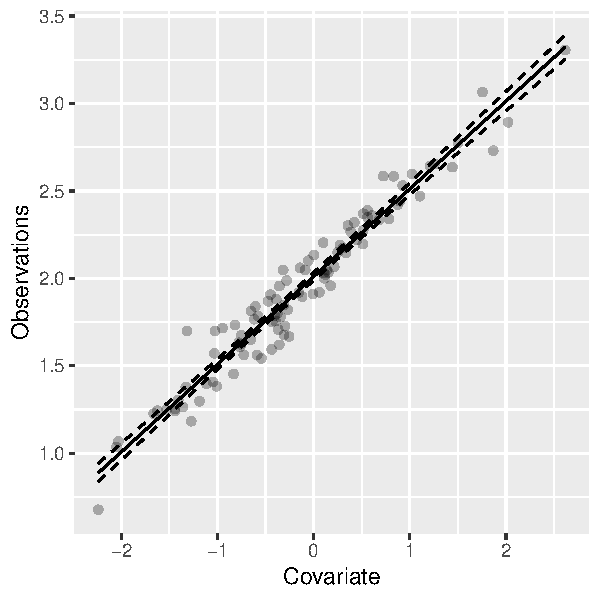
\includegraphics{practical1_compiler_files/figure-pdf/unnamed-chunk-11-1.pdf}

}

\caption{Data and 95\% credible intervals}

\end{figure}%

\subsection{R Code}

\begin{Shaded}
\begin{Highlighting}[]
\NormalTok{pred }\SpecialCharTok{\%\textgreater{}\%} \FunctionTok{ggplot}\NormalTok{() }\SpecialCharTok{+} 
  \FunctionTok{geom\_point}\NormalTok{(}\FunctionTok{aes}\NormalTok{(x,y), }\AttributeTok{alpha =} \FloatTok{0.3}\NormalTok{) }\SpecialCharTok{+}
  \FunctionTok{geom\_line}\NormalTok{(}\FunctionTok{aes}\NormalTok{(x,mean)) }\SpecialCharTok{+}
  \FunctionTok{geom\_line}\NormalTok{(}\FunctionTok{aes}\NormalTok{(x, q0}\FloatTok{.025}\NormalTok{), }\AttributeTok{linetype =} \StringTok{"dashed"}\NormalTok{)}\SpecialCharTok{+}
  \FunctionTok{geom\_line}\NormalTok{(}\FunctionTok{aes}\NormalTok{(x, q0}\FloatTok{.975}\NormalTok{), }\AttributeTok{linetype =} \StringTok{"dashed"}\NormalTok{)}\SpecialCharTok{+}
  \FunctionTok{xlab}\NormalTok{(}\StringTok{"Covariate"}\NormalTok{) }\SpecialCharTok{+} \FunctionTok{ylab}\NormalTok{(}\StringTok{"Observations"}\NormalTok{)}
\end{Highlighting}
\end{Shaded}

\begin{tcolorbox}[enhanced jigsaw, leftrule=.75mm, toprule=.15mm, bottomtitle=1mm, breakable, coltitle=black, arc=.35mm, titlerule=0mm, opacitybacktitle=0.6, left=2mm, rightrule=.15mm, colbacktitle=quarto-callout-warning-color!10!white, opacityback=0, colframe=quarto-callout-warning-color-frame, toptitle=1mm, colback=white, title={Task}, bottomrule=.15mm]

Generate predictions for a new observation with \(x_0 = 0.45\)

Take hint

You can create a new data frame containing the new observation \(x_0\)
and then use the \texttt{predict} function.

Click here to see the solution

\begin{Shaded}
\begin{Highlighting}[]
\NormalTok{new\_data }\OtherTok{=} \FunctionTok{data.frame}\NormalTok{(}\AttributeTok{x =} \FloatTok{0.45}\NormalTok{)}
\NormalTok{pred }\OtherTok{=} \FunctionTok{predict}\NormalTok{(fit.lm, new\_data, }\SpecialCharTok{\textasciitilde{}}\NormalTok{ beta\_0 }\SpecialCharTok{+}\NormalTok{ beta\_1,}
               \AttributeTok{n.samples =} \DecValTok{1000}\NormalTok{)}
\end{Highlighting}
\end{Shaded}

\end{tcolorbox}

\subsection{Generalized Linear Model}\label{sec-genlinmodel}

In this practical we will:

\begin{itemize}
\tightlist
\item
  Simulate non-Gaussian data
\item
  Learn how to fit a generalised linear model with \texttt{inlabru}
\item
  Generate predictions from the model
\end{itemize}

A generalised linear model allows for the data likelihood to be
non-Gaussian. In this example we have a discrete response variable which
we model using a Poisson distribution. Thus, we assume that our data \[
y_i \sim \text{Poisson}(\lambda_i)
\] with rate parameter \(\lambda_i\) which, using a log link, has
associated predictor \[
\eta_i = \log \lambda_i = \beta_0 + \beta_1 x_i 
\] with parameters \(\beta_0\) and \(\beta_1\), and covariate \(x\).
This is identical in form to the predictor in
Section~\ref{sec-linmodel}. The only difference is now we must specify a
different data likelihood.

\subsubsection{\texorpdfstring{\textbf{Simulate example
data}}{Simulate example data}}\label{simulate-example-data-1}

This code generates 100 samples of covariate \texttt{x} and data
\texttt{y}.

\begin{Shaded}
\begin{Highlighting}[]
\FunctionTok{set.seed}\NormalTok{(}\DecValTok{123}\NormalTok{)}
\NormalTok{n }\OtherTok{=} \DecValTok{100}
\NormalTok{beta }\OtherTok{=} \FunctionTok{c}\NormalTok{(}\DecValTok{1}\NormalTok{,}\DecValTok{1}\NormalTok{)}
\NormalTok{x }\OtherTok{=} \FunctionTok{rnorm}\NormalTok{(n)}
\NormalTok{lambda }\OtherTok{=} \FunctionTok{exp}\NormalTok{(beta[}\DecValTok{1}\NormalTok{] }\SpecialCharTok{+}\NormalTok{ beta[}\DecValTok{2}\NormalTok{] }\SpecialCharTok{*}\NormalTok{ x)}
\NormalTok{y }\OtherTok{=} \FunctionTok{rpois}\NormalTok{(n, }\AttributeTok{lambda  =}\NormalTok{ lambda)}
\NormalTok{df }\OtherTok{=} \FunctionTok{data.frame}\NormalTok{(}\AttributeTok{y =}\NormalTok{ y, }\AttributeTok{x =}\NormalTok{ x)  }
\end{Highlighting}
\end{Shaded}

\subsubsection{\texorpdfstring{Fitting a GLM in
\texttt{inlabru}}{Fitting a GLM in inlabru}}\label{fitting-a-glm-in-inlabru}

\begin{center}\rule{0.5\linewidth}{0.5pt}\end{center}

\textbf{Define model components and likelihood}

Since the predictor is the same as Section~\ref{sec-linmodel}, we can
use the same component definition:

\begin{Shaded}
\begin{Highlighting}[]
\NormalTok{cmp }\OtherTok{=}  \ErrorTok{\textasciitilde{}} \SpecialCharTok{{-}}\DecValTok{1} \SpecialCharTok{+} \FunctionTok{beta\_0}\NormalTok{(}\DecValTok{1}\NormalTok{) }\SpecialCharTok{+} \FunctionTok{beta\_1}\NormalTok{(x, }\AttributeTok{model =} \StringTok{"linear"}\NormalTok{)}
\end{Highlighting}
\end{Shaded}

However, when building the observation model likelihood we must now
specify the Poisson likelihood using the \texttt{family} argument (the
default link function for this family is the \(\log\) link).

\begin{Shaded}
\begin{Highlighting}[]
\NormalTok{lik }\OtherTok{=}  \FunctionTok{bru\_obs}\NormalTok{(}\AttributeTok{formula =}\NormalTok{ y }\SpecialCharTok{\textasciitilde{}}\NormalTok{.,}
            \AttributeTok{family =} \StringTok{"poisson"}\NormalTok{,}
            \AttributeTok{data =}\NormalTok{ df)}
\end{Highlighting}
\end{Shaded}

\textbf{Fit the model}

Once the likelihood object is constructed, fitting the model is exactly
the same process as in Section~\ref{sec-linmodel}.

\begin{Shaded}
\begin{Highlighting}[]
\NormalTok{fit\_glm }\OtherTok{=} \FunctionTok{bru}\NormalTok{(cmp, lik)}
\end{Highlighting}
\end{Shaded}

And model summaries can be viewed using

\begin{Shaded}
\begin{Highlighting}[]
\FunctionTok{summary}\NormalTok{(fit\_glm)}
\end{Highlighting}
\end{Shaded}

\begin{verbatim}
inlabru version: 2.12.0
INLA version: 24.06.27
Components:
beta_0: main = linear(1), group = exchangeable(1L), replicate = iid(1L), NULL
beta_1: main = linear(x), group = exchangeable(1L), replicate = iid(1L), NULL
Likelihoods:
  Family: 'poisson'
    Tag: ''
    Data class: 'data.frame'
    Response class: 'integer'
    Predictor: y ~ .
    Used components: effects[beta_0, beta_1], latent[]
Time used:
    Pre = 0.395, Running = 0.301, Post = 0.0729, Total = 0.769 
Fixed effects:
        mean    sd 0.025quant 0.5quant 0.975quant  mode kld
beta_0 0.915 0.071      0.775    0.915      1.054 0.915   0
beta_1 1.048 0.056      0.938    1.048      1.157 1.048   0

Deviance Information Criterion (DIC) ...............: 386.39
Deviance Information Criterion (DIC, saturated) ....: 120.67
Effective number of parameters .....................: 2.00

Watanabe-Akaike information criterion (WAIC) ...: 387.33
Effective number of parameters .................: 2.73

Marginal log-Likelihood:  -204.02 
 is computed 
Posterior summaries for the linear predictor and the fitted values are computed
(Posterior marginals needs also 'control.compute=list(return.marginals.predictor=TRUE)')
\end{verbatim}

\subsubsection{Generate model
predictions}\label{generate-model-predictions-1}

\begin{center}\rule{0.5\linewidth}{0.5pt}\end{center}

To generate new predictions we must provide a data frame that contains
the covariate values for \(x\) at which we want to predict.

This code block generates predictions for the data we used to fit the
model (contained in \texttt{df\$x}) as well as 10 new covariate values
sampled from a uniform distribution \texttt{runif(10)}.

\begin{Shaded}
\begin{Highlighting}[]
\CommentTok{\# Define new data, set to NA the values for prediction}

\NormalTok{new\_data }\OtherTok{=} \FunctionTok{data.frame}\NormalTok{(}\AttributeTok{x =} \FunctionTok{c}\NormalTok{(df}\SpecialCharTok{$}\NormalTok{x, }\FunctionTok{runif}\NormalTok{(}\DecValTok{10}\NormalTok{)),}
                      \AttributeTok{y =} \FunctionTok{c}\NormalTok{(df}\SpecialCharTok{$}\NormalTok{y, }\FunctionTok{rep}\NormalTok{(}\ConstantTok{NA}\NormalTok{,}\DecValTok{10}\NormalTok{)))}

\CommentTok{\# Define predictor formula}
\NormalTok{pred\_fml }\OtherTok{\textless{}{-}} \ErrorTok{\textasciitilde{}} \FunctionTok{exp}\NormalTok{(beta\_0 }\SpecialCharTok{+}\NormalTok{ beta\_1)}

\CommentTok{\# Generate predictions}
\NormalTok{pred\_glm }\OtherTok{\textless{}{-}} \FunctionTok{predict}\NormalTok{(fit\_glm, new\_data, pred\_fml)}
\end{Highlighting}
\end{Shaded}

Since we used a log link (which is the default for
\texttt{family\ =\ "poisson"}), we want to predict the exponential of
the predictor. We specify this using a general \texttt{R} expression
using the formula syntax.

\begin{tcolorbox}[enhanced jigsaw, leftrule=.75mm, toprule=.15mm, bottomtitle=1mm, breakable, coltitle=black, arc=.35mm, titlerule=0mm, opacitybacktitle=0.6, left=2mm, rightrule=.15mm, colbacktitle=quarto-callout-note-color!10!white, opacityback=0, colframe=quarto-callout-note-color-frame, toptitle=1mm, colback=white, title=\textcolor{quarto-callout-note-color}{\faInfo}\hspace{0.5em}{Note}, bottomrule=.15mm]

Note that the \texttt{predict} function will call the component names
(i.e.~the ``labels'') that were decided when defining the model.

\end{tcolorbox}

Since the component definition is looking for a covariate named \(x\),
all we need to provide is a data frame that contains one, and the
software does the rest.

\subsection{Plot}

\begin{figure}[H]

{\centering 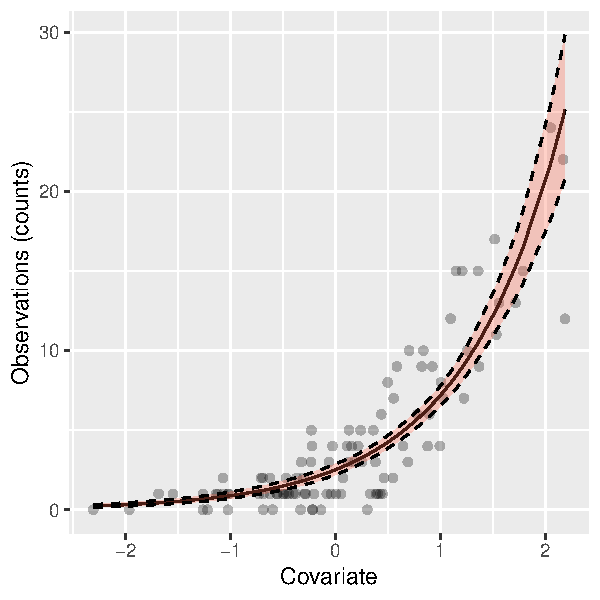
\includegraphics{practical1_compiler_files/figure-pdf/unnamed-chunk-34-1.pdf}

}

\caption{Data and 95\% credible intervals}

\end{figure}%

\subsection{R Code}

\begin{Shaded}
\begin{Highlighting}[]
\NormalTok{pred\_glm }\SpecialCharTok{\%\textgreater{}\%} \FunctionTok{ggplot}\NormalTok{() }\SpecialCharTok{+} 
  \FunctionTok{geom\_point}\NormalTok{(}\FunctionTok{aes}\NormalTok{(x,y), }\AttributeTok{alpha =} \FloatTok{0.3}\NormalTok{) }\SpecialCharTok{+}
  \FunctionTok{geom\_line}\NormalTok{(}\FunctionTok{aes}\NormalTok{(x,mean)) }\SpecialCharTok{+}
    \FunctionTok{geom\_ribbon}\NormalTok{(}\FunctionTok{aes}\NormalTok{(}\AttributeTok{x =}\NormalTok{ x, }\AttributeTok{ymax =}\NormalTok{ q0}\FloatTok{.975}\NormalTok{, }\AttributeTok{ymin =}\NormalTok{ q0}\FloatTok{.025}\NormalTok{),}\AttributeTok{fill =} \StringTok{"tomato"}\NormalTok{, }\AttributeTok{alpha =} \FloatTok{0.3}\NormalTok{)}\SpecialCharTok{+}
  \FunctionTok{xlab}\NormalTok{(}\StringTok{"Covariate"}\NormalTok{) }\SpecialCharTok{+} \FunctionTok{ylab}\NormalTok{(}\StringTok{"Observations (counts)"}\NormalTok{)}
\end{Highlighting}
\end{Shaded}

\begin{tcolorbox}[enhanced jigsaw, leftrule=.75mm, toprule=.15mm, bottomtitle=1mm, breakable, coltitle=black, arc=.35mm, titlerule=0mm, opacitybacktitle=0.6, left=2mm, rightrule=.15mm, colbacktitle=quarto-callout-warning-color!10!white, opacityback=0, colframe=quarto-callout-warning-color-frame, toptitle=1mm, colback=white, title={Task}, bottomrule=.15mm]

Suppose a binary response such that

\[
    \begin{aligned}
y_i &\sim \mathrm{Bernoulli}(\psi_i)\\
\eta_i &= \mathrm{logit}(\psi_i) = \alpha_0 +\alpha_1 \times w_i 
\end{aligned}
\] Using the following simulated data, use \texttt{inlabru} to fit the
logistic regression above. Then, plot the predictions for the data used
to fit the model along with 10 new covariate values

\begin{Shaded}
\begin{Highlighting}[]
\FunctionTok{set.seed}\NormalTok{(}\DecValTok{123}\NormalTok{)}
\NormalTok{n }\OtherTok{=} \DecValTok{100}
\NormalTok{alpha }\OtherTok{=} \FunctionTok{c}\NormalTok{(}\FloatTok{0.5}\NormalTok{,}\FloatTok{1.5}\NormalTok{)}
\NormalTok{w }\OtherTok{=} \FunctionTok{rnorm}\NormalTok{(n)}
\NormalTok{psi }\OtherTok{=} \FunctionTok{plogis}\NormalTok{(alpha[}\DecValTok{1}\NormalTok{] }\SpecialCharTok{+}\NormalTok{ alpha[}\DecValTok{2}\NormalTok{] }\SpecialCharTok{*}\NormalTok{ w)}
\NormalTok{y }\OtherTok{=} \FunctionTok{rbinom}\NormalTok{(}\AttributeTok{n =}\NormalTok{ n, }\AttributeTok{size =} \DecValTok{1}\NormalTok{, }\AttributeTok{prob =}\NormalTok{  psi) }\CommentTok{\# set size = 1 to draw binary observations}
\NormalTok{df\_logis }\OtherTok{=} \FunctionTok{data.frame}\NormalTok{(}\AttributeTok{y =}\NormalTok{ y, }\AttributeTok{w =}\NormalTok{ w)  }
\end{Highlighting}
\end{Shaded}

Here we use the logit link function
\(\mathrm{logit}(x) = \log\left(\frac{x}{1-x}\right)\)
(\texttt{plogis()} function in R) to link the linear predictor to the
probabilities \(\psi\).

Take hint

You can set \texttt{family\ =\ "binomial"} for binary responses and the
\texttt{plogis()} function for computing the predicted values.

\begin{tcolorbox}[enhanced jigsaw, leftrule=.75mm, toprule=.15mm, bottomtitle=1mm, breakable, coltitle=black, arc=.35mm, titlerule=0mm, opacitybacktitle=0.6, left=2mm, rightrule=.15mm, colbacktitle=quarto-callout-note-color!10!white, opacityback=0, colframe=quarto-callout-note-color-frame, toptitle=1mm, colback=white, title=\textcolor{quarto-callout-note-color}{\faInfo}\hspace{0.5em}{Note}, bottomrule=.15mm]

The Bernoulli distribution is equivalent to a
\(\mathrm{Binomial}(1, \psi)\) pmf. If you have proportional data
(e.g.~no. successes/no. trials) you can specify the number of events as
your response and then the number of trials via the
\texttt{Ntrials\ =\ n} argument of the \texttt{bru\_obs} function (where
\texttt{n} is the known vector of trials in your data set).

\end{tcolorbox}

Click here to see the solution

\begin{Shaded}
\begin{Highlighting}[]
\CommentTok{\# Model components}
\NormalTok{cmp\_logis }\OtherTok{=}  \ErrorTok{\textasciitilde{}} \SpecialCharTok{{-}}\DecValTok{1} \SpecialCharTok{+} \FunctionTok{alpha\_0}\NormalTok{(}\DecValTok{1}\NormalTok{) }\SpecialCharTok{+} \FunctionTok{alpha\_1}\NormalTok{(w, }\AttributeTok{model =} \StringTok{"linear"}\NormalTok{)}
\CommentTok{\# Model likelihood}
\NormalTok{lik\_logis }\OtherTok{=}  \FunctionTok{bru\_obs}\NormalTok{(}\AttributeTok{formula =}\NormalTok{ y }\SpecialCharTok{\textasciitilde{}}\NormalTok{.,}
            \AttributeTok{family =} \StringTok{"binomial"}\NormalTok{,}
            \AttributeTok{data =}\NormalTok{ df\_logis)}
\CommentTok{\# fit the model}
\NormalTok{fit\_logis }\OtherTok{\textless{}{-}} \FunctionTok{bru}\NormalTok{(cmp\_logis,lik\_logis)}

\CommentTok{\# Define data for prediction}
\NormalTok{new\_data }\OtherTok{=} \FunctionTok{data.frame}\NormalTok{(}\AttributeTok{w =} \FunctionTok{c}\NormalTok{(df\_logis}\SpecialCharTok{$}\NormalTok{w, }\FunctionTok{runif}\NormalTok{(}\DecValTok{10}\NormalTok{)),}
                      \AttributeTok{y =} \FunctionTok{c}\NormalTok{(df\_logis}\SpecialCharTok{$}\NormalTok{y, }\FunctionTok{rep}\NormalTok{(}\ConstantTok{NA}\NormalTok{,}\DecValTok{10}\NormalTok{)))}
\CommentTok{\# Define predictor formula}
\NormalTok{pred\_fml }\OtherTok{\textless{}{-}} \ErrorTok{\textasciitilde{}} \FunctionTok{plogis}\NormalTok{(alpha\_0 }\SpecialCharTok{+}\NormalTok{ alpha\_1)}

\CommentTok{\# Generate predictions}
\NormalTok{pred\_logis }\OtherTok{\textless{}{-}} \FunctionTok{predict}\NormalTok{(fit\_logis, new\_data, pred\_fml)}

\CommentTok{\# Plot predictions}
\NormalTok{pred\_logis }\SpecialCharTok{\%\textgreater{}\%} \FunctionTok{ggplot}\NormalTok{() }\SpecialCharTok{+} 
  \FunctionTok{geom\_point}\NormalTok{(}\FunctionTok{aes}\NormalTok{(w,y), }\AttributeTok{alpha =} \FloatTok{0.3}\NormalTok{) }\SpecialCharTok{+}
  \FunctionTok{geom\_line}\NormalTok{(}\FunctionTok{aes}\NormalTok{(w,mean)) }\SpecialCharTok{+}
    \FunctionTok{geom\_ribbon}\NormalTok{(}\FunctionTok{aes}\NormalTok{(}\AttributeTok{x =}\NormalTok{ w, }\AttributeTok{ymax =}\NormalTok{ q0}\FloatTok{.975}\NormalTok{, }\AttributeTok{ymin =}\NormalTok{ q0}\FloatTok{.025}\NormalTok{),}\AttributeTok{fill =} \StringTok{"tomato"}\NormalTok{, }\AttributeTok{alpha =} \FloatTok{0.3}\NormalTok{)}\SpecialCharTok{+}
  \FunctionTok{xlab}\NormalTok{(}\StringTok{"Covariate"}\NormalTok{) }\SpecialCharTok{+} \FunctionTok{ylab}\NormalTok{(}\StringTok{"Observations"}\NormalTok{)}
\end{Highlighting}
\end{Shaded}

\begin{center}
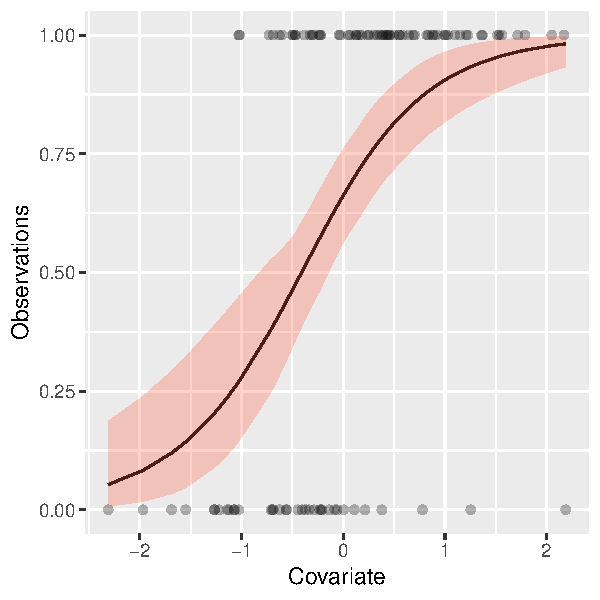
\includegraphics{practical1_compiler_files/figure-pdf/unnamed-chunk-37-1.pdf}
\end{center}

\end{tcolorbox}



\end{document}
